%% The following is a directive for TeXShop to indicate the main file
%%!TEX root = diss.tex
\chapter{Background and roadmap}
\label{ch:Introduction}

\begin{itemize}
    \item Optimization approaches have enjoyed prominence in machine learning, data mining and signal processing because of their wide applicability and attractive theoretical properties.
    \item Optimization formulations and methods are proving to be vital in designing algorithms to extract essential knowledge from huge volumes of data. 
    \item For a long time, it has been recognized that looking at the dual of an optimization problem may drastically simplify its solution or enjoy better convergence rate.
    \item In this thesis, we focus on the effectiveness of duality in two classes of optimization problems: structured optimization and federated optimization. 
\end{itemize}

  

\section{Basic definitions and notations} \label{sec:1-1}

In this section, we introduce some basic notations and definitions that will be used in this thesis. We use capital letters $A, B, \dots$ to denote matrices or linear operators, lowercase letters $a, b, \dots$ to denote vectors, calligraphic letters $\Ascr, \Bscr, \dots$ to denote sets, and Greek letters $\alpha, \beta, \dots$ to denote scalars.

We work with $n$-vectors in $\Real^n$ and $p$-by-$n$ matrices in $\Real^{p\times
n}$. The restriction to real-valued vectors and matrices considerably simplifies
our development, though many of the ideas set forth in this thesis extend to
more general functional spaces, as described by \citet{zalinescu2002convex} and
\citet{bauschke2011convex}.

Let $e_i$ denote the $i$th canonical unit vector, i.e., the vector of all zeros
except a single 1 in the $i$th position. The dot product of two $n$-vectors $x$
and $z$ is $\ip x z = \sum_{j} x_j z_j$. The dot product of two $p$-by-$n$
matrices $X$ and $Z$ is the trace inner product $\ip X Z = \trace(X\T Z) =
\sum_{ij}X_{ij}Z_{ij}$.

A vector norm $\|x\|$ always refers to the 2-norm, i.e., $\|x\| = \sqrt{\ip{x}{x}}$ unless otherwise specified. Matrix norms always refer to the Schatten norm, e.g., if $(s_1, s_2,\ldots)$ are
the singular values of $X$, then
\[
  \|X\|_1 = \sum_i s_i,
  \quad \|X\|_2=\Big(\sum_i s_i^2\Big)^{1/2},
  \text{and} \|X\|_\infty=\max_i s_i.
\]

The adjoint $M^*$ of any linear map $M$ is the unique
linear map that satisfies the relationship $\ip{Mx}{z}=\ip{x}{M^*z}$ for all $x$ and $z$. Thus, for
the linear map $M:\Real^n\to\Real^m$, the product of the adjoint and an
$m$-vector $y$ is $M^*y = \sum_{i=1}^m y_i (Me_i)$. For the linear map
$M:\Real^{p\times n}\to\Real^m$, the forward and adjoint maps take the form
\begin{equation} \label{eq:mat-map}
  M X = \begin{bmatrix}
    \ip{M_1}{X} \\ \vdots \\ \ip{M_m}{X}
  \end{bmatrix}  
  \quad\mbox{and}\quad
  M^*y = \sum_{i=1}^m y_i M_i,
\end{equation}
where each $M_i$ is a $p$-by-$n$ matrix. The notation $X\succeq0$
indicates that $X$ is symmetric positive definite.

A set $\Cscr$ is convex if
\[
    \begin{cases}
        \lambda &\in [0,1]\\
        x &\in \Cscr\\
        y &\in \Cscr
    \end{cases}
    \Rightarrow 
    \lambda x + (1-\lambda)y \in \Cscr. 
\]
For any convex set $\Cscr$, its polar set is given by 
\begin{equation} \label{eq-polar-set}
    \Cscr\polar=\{z | \ip x z \le 1 \mbox{\ for all\ } x\in\Cscr \}.
\end{equation}
The indicator to $\Cscr$ is the
function
\[
  \delta\Cs(x) = \begin{cases}
    0 & \mbox{if $x\in\Cscr$;}
\\ +\infty & \mbox{otherwise}.
  \end{cases}
\]
The normal cone to $\Cscr$ at $x\in\Cscr$ is defined as
\[\Nscr\Cs(x) = \{d \mid \ip{d}{u - x} \leq 0 \mbox{ for all } u \in \Cscr\}.\]
The Euclidean projection onto $\Cscr$ is denoted
\[\proj\Cs(x) = \argmin{u \in \Cscr} \ \|x - u\|_2,\]
which defines the distance of a point to the set $\Cscr$, denoted by
\[\dist\Cs(x) = \|x - \proj\Cs(x)\|_2.\]

For any set $\Ascr$, its convex hull contains all
weighted averages of the elements of the set, denoted
\[
  \conv \Ascr =
  \left\{\sum_{i=1}^m \alpha_i x_i ~\bigg\vert~ x_i\in\Ascr,\ \alpha_i\ge0,\ \sum_{i=1}^m\alpha_i=1 \right\},
\]
for some some positive integer $m$. The conic extension of $\Ascr$ is defined by 
\[
  \cone\Ascr = \{\alpha d ~|~ d\in\Ascr,\ \alpha\ge0\}.
\]
The closure, boundary and relative interior, respectively,
of $\Ascr$ denoted $\cl\Ascr$, $\bnd\Ascr$ and $\ri\Ascr$. 
The gauge function with respect to $\Ascr$ is defined as the Minkowski functional to the closed convex hull of $\Ascr$, i.e.,
\begin{equation} \label{eq:gauge1}
    \gauge\As(x) = \inf\left\{\mu > 0 ~|~ x \in \mu\cl\conv(\Ascr\cup\{0\})\right\}.
\end{equation}
The support function with respect to $\Ascr$ is defined as 
\begin{equation} \label{eq:support}
    \sigma\As(z) = \sup\{\ip{a}{z} ~|~ a\in\Ascr\cup\{0\}\}.
\end{equation}
The descent cone of the set $\Ascr$ at point $x$ is defined as 
\[\Dscr(\Ascr, x) = \cone\{d\in \Re^n ~|~ \gauge\As(x + d) \leq \gauge\As(x)\}\]

Let $\Nscr(0,I)$ denote the standard Gaussian distribution. For a compact set $\Sscr$, $\uniform(\Sscr)$ denotes the uniform ditribution over $\Sscr$. For a convex cone $\Dscr$, let $\delta(\Dscr) \coloneqq \mE_{g\sim\Nscr(0,I)} \|\proj_{\Dscr}(g)\|_2^2 $ denote the statistical dimension of the cone $\Dscr$.

Consider a differentiable function $f:\Real^n\to\Real\cup\{+\infty\}$. The function $f$ is convex if $f$ satisfies
\[f(y) \geq f(y) + \ip{\nabla f(x)}{y-x} \enspace \forall x, y \in \Re^n.\]
The function $f$ is $\alpha$-strongly convex for some $\alpha>0$ if $f$ satisfies
\[f(y) \geq f(x) + \ip{\nabla f(x)}{y-x} + \frac{\alpha}{2}\|x-y\|^2 \enspace \forall x, y \in \Re^n.\]
The function $f$ is $\beta$-smooth for some $\beta>0$ if $f$ satisfies
\[f(y) \leq f(x) + \ip{\nabla f(x)}{y-x} + \frac{\beta}{2}\|x-y\|^2 \enspace \forall x, y \in \Re^n.\]
The function $f$ is $\vartheta$-Lipschitz for some $\vartheta>0$ if $f$ satisfies
\[|f(x) - f(y)| \leq \vartheta\|x-y\| \enspace \forall x, y \in \Re^n.\]
The domain is denoted
$\dom f = \{x~|~f(x)<+\infty\}$, and the convex conjugate is denoted
\[
  f^*(z) = \sup_{x\in\Re^n}\{\ip x z - f(x) \}.
\] 


\section{Duality in optimization} \label{sec:1-2}

Modern treatment of duality in convex optimization is based on an interpretation of multipliers as giving sensitivity information relative to perturbations in the problem data. The perturbation framework pioneered by \citet{rockafellar1970convex} plays an important rule in the duality theory. Here we briefly summarize this framework. 

Consider a general convex optimization problem
\begin{equation} \label{prob:general_cvx}
    \minimize{x \in \Re^n} f(x),
\end{equation}
where $f:\Re^n \to \Re$ is a closed convex function. The perturbation framework depends on an arbitrary convex perturbation function $F: \Re^n \times \Re^m \to \Re$ such that 
\begin{equation} \label{eq:value_fn_property}
    F(x, 0) = f(x) \enspace \forall x \in \Re^n.
\end{equation}
The corresponding value function $v_F : \Re^m \to \Re$ is given by 
\begin{equation}
    v_F(u) = \inf_{x \in \Re^n} F(x, u).
\end{equation}
This set-up immediately yields the primal-dual pair
\begin{align}
    v_F(0) &= \inf_{x \in \Re^n} F(x, 0), \label{prob:general_primal}\\
    v_F^{**}(0) &= \sup_{y \in \Re^m} -F^*(0, y). \label{prob:general_dual}
\end{align}
By the property~\eqref{eq:value_fn_property} of the perturbation function $F$, we can see that problem~\eqref{prob:general_primal} is equivalent to the general convex optimization problem~\eqref{prob:general_cvx}. The problem~\eqref{prob:general_dual} is known as the \emph{dual} problem of~\eqref{prob:general_cvx} corresponding to the perturbation function $F$. 
The following theorem, developed by \citet{rockafellar1998variational}, describes the relationship between the primal-dual pair:~\eqref{prob:general_primal} and~\eqref{prob:general_dual}. 

\begin{theorem}[Weak and strong duality~\protect{\citep[Theorem~11.39]{rockafellar1998variational}}] Consider the primal-dual pair:~\eqref{prob:general_primal} and~\eqref{prob:general_dual}, where $F: \Re^n \times \Re^m \to \Re$ is a proper, closed and convex function. The following properties hold. 
    \begin{itemize}
        \item \textbf{Weak duality}. The inequality $v_F(0) \geq v_F^{**}(0)$ always holds. 
        \item \textbf{Strong duality}. If $0 \in \ri\dom v_F \cup \ri\dom v_F^{**}$, then $v_F(0) = v_F^{**}(0)$. 
        \item \textbf{Optimal solutions.} If the strong duality holds with finite optimal values, then the following characterizations of the optimal solutions to the primal-dual pair are equivalent
            \begin{align}
                (x^*, 0) &\in \partial F^*(0,y^*); \\
                (0, y^*) &\in \partial F(x^*,0); \\
                v_F(0) = F^*(x^*, 0) &= -F^*(0,y^*) = v_F^{**}(0).
            \end{align}
    \end{itemize}
\end{theorem}

The perturbation function $F$ plays an important role in Fenchel-Rockafellar duality theory. Different choices of the perturbation function will lead to different dual problems. In the rest of this section, I will introduce three widely used primal-dual pairs: Lagrange dual, Fenchel dual and gauge dual. 


\subsection{Lagrangian dual}
Consider the general constrained convex optimization problem:
\begin{equation} \label{prob:general_constrained} 
    \minimize{x \in \Re^n} f(x) \st c_i(x) \leq 0 \enspace \forall i = 1, \dots, m,
\end{equation}
where $f:\Re^n\to\Re$ and $c_i:\Re^n\to\Re$ for all $i\in[m]$ are convex functions. In this case, the perturbation function is defined as 
\begin{equation}
    F(x, u) = f(x) + \sum_{i = 1}^m \delta_{\leq 0}(c_i(x) + u_i).
\end{equation}
Then we can derive the corresponding conjugate function as 
\begin{align*}
    -F^*(0, y) &= -\sup_{x\in\Re^n, u\in\Re^m} \ip{0}{x} + \ip{y}{u} - F(x,u)
             \\&= -\sup_{x\in\Re^n, w\in\Re_+^m} \sum_{i=1}^m \ip{y_i}{- c_i(x) - w_i} - f(x)
             \\&= 
             \begin{cases}
                 \inf_{x\in\Re^n} f(x) + \sum_{i=1}^m \ip{y_i}{c_i(x)} & \text{if} y \in\Re_+^m \\
                 -\infty & \text{otherwise}.
             \end{cases}
\end{align*}
Therefore, the Lagrangian dual to problem~\eqref{prob:general_constrained} is given by
\begin{equation} \label{prob:general_constrained_dual}
    \maximize{y\in\Re_+^m} \minimize{x \in \Re^n} f(x) + \sum_{i=1}^m \ip{y_i}{c_i(x)}.
\end{equation}
The following theorem characterizes the duality for the Lagrangian primal-dual pair. 

\begin{theorem}[Lagrangian duality] 
    Let $p^*$ and $d^*$ denote respectively the optimal values for the Lagrangian primal-dual pair:~\eqref{prob:general_constrained} and~\eqref{prob:general_constrained_dual}. 
    \item \textbf{Weak duality}. $p^* \geq d^*$. 
    \item \textbf{Strong duality}. 
    If there exist an interior-point feasible point $\hat x$ for the primal problem~\eqref{prob:general_constrained}, i.e. $c_i(\hat x) < 0$ for $i = 1,\dots,m$, then $p^* = d^*$. Furthermore, let $x^*$ and $y^*$ denote respectively the optimal solutions to the primal-dual pair:~\eqref{prob:general_constrained} and~\eqref{prob:general_constrained_dual}, then 
    \[y_i^*c_i(x^*) = 0 \enspace \forall i = 1,\dots,m.\]
\end{theorem}


\subsection{Fenchel duality}
Consider the following optimization problem 
\begin{equation} \label{prob:general_fenchel} 
    \minimize{x \in \Re^n} f(x) + g(Mx),
\end{equation}
where $f:\Re^n\to\Re$ and $g:\Re^m\to\Re$ are closed convex functions, and $M:\Re^n\to\Re^m$ is a linear operator. In this case, the perturbation function is defined as 
\begin{equation}
    F(x, u) = f(x) + g(Mx + u).
\end{equation}
Then we can derive the corresponding conjugate function as
\begin{align*}
    -F^*(0, y) &= -\sup_{x\in\Re^n, u\in\Re^m} \ip{0}{x} + \ip{y}{u} - f(x) - g(Mx + u)
             \\&= -\sup_{x\in\Re^n} \left\{\sup_{u\in\Re^m} \ip{y}{Mx + u} - g(Mx + u)\right\} - f(x) - \ip{y}{Mx}
             \\&= - g^*(y) - \sup_{x\in\Re^n}\ip{-M^*y}{x} - f(x) 
             \\&= - g^*(y) - f(-M^*y).
\end{align*}
Therefore, the Fenchel dual to problem~\eqref{prob:general_fenchel} is given by
\begin{equation} \label{prob:general_fenchel_dual}
    \maximize{y\in\Re^m} - g^*(y) - f(-M^*y).
\end{equation}
The following theorem characterizes the duality for the Fenchel primal-dual pair. 

\begin{theorem}[Fenchel duality] 
    Let $p^*$ and $d^*$ denote respectively the optimal values for the Fenchel primal-dual pair:~\eqref{prob:general_fenchel} and~\eqref{prob:general_fenchel_dual}. 
    \item \textbf{Weak duality}. $p^* \geq d^*$. 
    \item \textbf{Strong duality}. 
    If $0\in\int(\dom g - M\dom f)$, then $p^* = d^*$. Furthermore, let $x^*$ and $y^*$ denote respectively the optimal solutions to the primal-dual pair:~\eqref{prob:general_fenchel} and~\eqref{prob:general_fenchel_dual}, then the following relationships hold
    \begin{align*}
          y^* &\in \partial g(Mx^*) \cap (M^*)^{-1}\partial f(x^*) \tand
        \\x^* &\in \partial f^*(-M^*y^*)\cap M^{-1}\partial g^*(y^*).
    \end{align*}
\end{theorem}




\subsection{Gauge duality}
Consider the following gauge optimization problem 
\begin{equation} \label{prob:general_gauge} 
    \minimize{x \in \Re^n} \gauge\Cs(x) \st Mx = b,
\end{equation}
where $\Cscr\subseteq\Re^n$ is a convex set and $\gauge\Cs$ is the corresponding gauge function, $M:\Re^n\to\Re^m$ is a linear operator, and $b\in\Re^m$ is a vector. By setting 
$\lambda \coloneqq 1/\gauge\Cs(x)$ and $w \coloneqq \lambda x$, problem~\eqref{prob:general_gauge} can be expressed as 
\begin{equation} \label{prob:general_gauge2} 
    \inf_{\lambda > 0, w \in \Re^n} \frac{1}{\lambda} \st w \in \Cscr \tand Mw = \lambda b.
\end{equation}
Note that minimizing $1/\lambda$ is equivalent to minimizing $-\lambda$ for $\lambda \geq 0$. In this case, the perturbation function is defined as 
\begin{equation}
    F(\lambda, w, u) = -\lambda + \delta\Cs(w) + \delta_{\{0\}}(\lambda b - Mw + u) + \delta_{\geq 0}(\lambda). 
\end{equation}
Then we can derive the corresponding conjugate function as
\begin{align*}
    -F^*(0, y) &= -\sup_{\lambda\in\Re, w\in\Re^n, u\in\Re^m} \ip{y}{u} + \lambda - \delta\Cs(w) - \delta_{\{0\}}(\lambda b - Mw + u) - \delta_{\geq 0}(\lambda)
    \\&= -\sup_{\lambda\in\Re, w\in\Re^n} \lambda - \delta\Cs(w) - \delta_{\geq 0}(\lambda) - \ip{\lambda b - Mw}{y}
    \\&= -\sup_{\lambda\geq 0} \delta\Cs^*(M^*y) + \lambda ( 1 - \ip{b}{y} )
    \\&= 
        \begin{cases}
            -\delta\Cs^*(M^*y) & \text{if} \ip{b}{y} \geq 1 \\
            -\infty & \text{otherwise}.
        \end{cases}
\end{align*}
Therefore, the gauge dual to problem~\eqref{prob:general_gauge} is given by
\begin{equation} \label{prob:general_gauge_dual}
    \maximize{y\in\Re^m} -\delta\Cs^*(M^*y) \st \ip{b}{y} \geq 1.
\end{equation}
The following theorem characterizes the duality for the gauge primal-dual pair. 

\begin{theorem}[Gauge duality] 
    Let $p^*$ and $d^*$ denote respectively the optimal values for the gauge primal-dual pair:~\eqref{prob:general_gauge} and~\eqref{prob:general_gauge_dual}. 
    \item \textbf{Weak duality}. If both primal problem~\eqref{prob:general_gauge} and dual problem~\eqref{prob:general_gauge_dual} are feasible, then $p^* d^* \geq 1$. 
    \item \textbf{Strong duality}. If either primal problem~\eqref{prob:general_gauge} or dual problem~\eqref{prob:general_gauge_dual} is strictly feasible and the other is feasible, then $p^* d^* = 1$. Furthermore, let $x^*$ and $y^*$ denote respectively the optimal solutions to the primal-dual pair:~\eqref{prob:general_gauge} and~\eqref{prob:general_gauge_dual}, then 
    \[\ip{x^*}{M^*y^*} = \gauge\Cs(x^*)\delta\Cs^*(M^*y^*).\]
    
\end{theorem}

\section{Structured optimization} \label{sec:1-3}

Convex optimization provides a valuable computational framework that renders many problems tractable because of the range of powerful algorithms that can be brought to the task. The key is that a certain mathematical structure, i.e., convexity of the functions and sets defining the problem—lays open an enormous range of theoretical and algorithmic tools that lend themeselves astonishingly well to computation. There are limits, however, to the scalability of general-purpose algorithms for convex optimization. As has been recognized in the optimization and related communities for at least the past decade, significant efficiencies can be gained by acknowledging the latent structure in the solution itself, coupled with the overarching structure provided by convexity.

Structured optimization proceeds along these lines by using a prescribed set of atoms from which to assemble an optimal solution. The atomic decomposition of a vector $x\in\Re^n$ with respect to an atomic set
$\Ascr\subset\Re^n$ is given by the weighted superposition
\begin{equation} \label{eq:atomic-decomp}
  x = \sum_{a\in\Ascr} c_a a, \quad c_a\ge0 \quad \forall a\in\Ascr.
\end{equation}
Each coefficient $c_a$ in the atomic decomposition measures the contribution of
the corresponding atom $a$ toward the representation of $x$. Intuitively, an
atomic decomposition reveals structural information implicit in a vector, with
large coefficients in the decomposition indicating the more significant
structures.

Within the context of an optimization problem, the atomic decomposition reveals
structural elements most significant in the minimization process.
In the simplest case, the atoms $\Ascr$ may be formed from the collection of
signed canonical unit vectors $\{\pm e_1,\ldots,\pm e_n\}$, which leads to the
atomic decomposition
\[
  x = \sum_{j=1}^n c_j a_j,
  \quad
  c_j: = |x_j|,
  \quad
  a_j:= (\sgn x_j)\cdot e_j.
\]
Trivially, the most significant atoms thus correspond to the variables $x_j$ in
the vector $x=(x_1,\ldots,x_n)$ with the largest magnitude.

This generic model for atomic decompositions was promoted by~\citet{cds98} in the context of sparse signal decomposition, and more recently, by~\citet{chandrasekaran2012convex}, who were concerned with obtaining sparse solutions to linear inverse problems. 

In this thesis, we want to answer the question of determining which of the atoms in the atomic set $\Ascr$ are essential to the atomic decomposition of $x$, and conversely, which atoms can be safely ignored. Our approach studies the atomic decomposition framework from a geometric perspective and is based on a certain duality correspondence particular to gauge functions and to convex cones that are implicit in their definition. We further show that this duality correspondence allows us to develop efficient and scalable algorithms for the structured optimization problems, and design new structured optimization model for real world applications. We provide a more detailed roadmap in \autoref{sec:1-4}. 

\section{Federated learning} \label{sec:1-4}

Building large and powerful machine learning models often needs large amounts of training data. In many industry-scale applications, training data is distributed in the form of silos, that is, training data is obtained and maintained by many data owners instead of being centralized at the place of a single owner or a data center. Because of industrial competition, privacy concerns, legal restrictions, and many other possible reasons, integrating or centralizing data from different sources faces enormous resistance and is often even infeasible~\cite{li2020review}. Federated learning, originally proposed by~\citet{federated2016}, is promising for training machine learning models on distributed data sources. It facilitates collaboration among a group of data owners (aka.~``clients'') and, at the same time, preserves their privacy. The central idea of federated learning is to periodically aggregate local models from clients to produce a more general and capable global model.

Federated learning can be further be classified into two main categories: horizontal federated learning and vertical federated learning~\cite{yang2019federated}. Broadly speaking, horizontal federated learning refers to the scenarios where various clients' data sets share the same feature space but have separate sample IDs, and vertical federated learning refers to the scenarios where data sets owned by different clients share the identical sample IDs but have distinctive features. A simple characterization is shown in \autoref{fig:hfl_and_vfl}. 

\begin{figure}[t] 
    \begin{subfigure}{.48\textwidth}
      \centering
      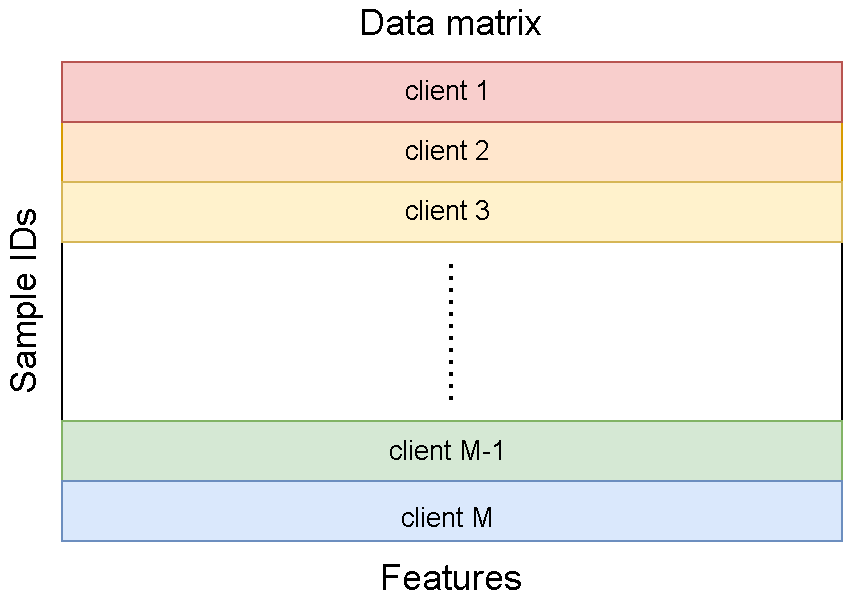
\includegraphics[width=\linewidth]{./figures/hfl_illustration.pdf}
      \captionsetup{justification=centering}
      \caption{Horizontal federated learning.}
      \label{fig:hfl}
    \end{subfigure}
    \hfill
    \begin{subfigure}{.48\textwidth}
      \centering
      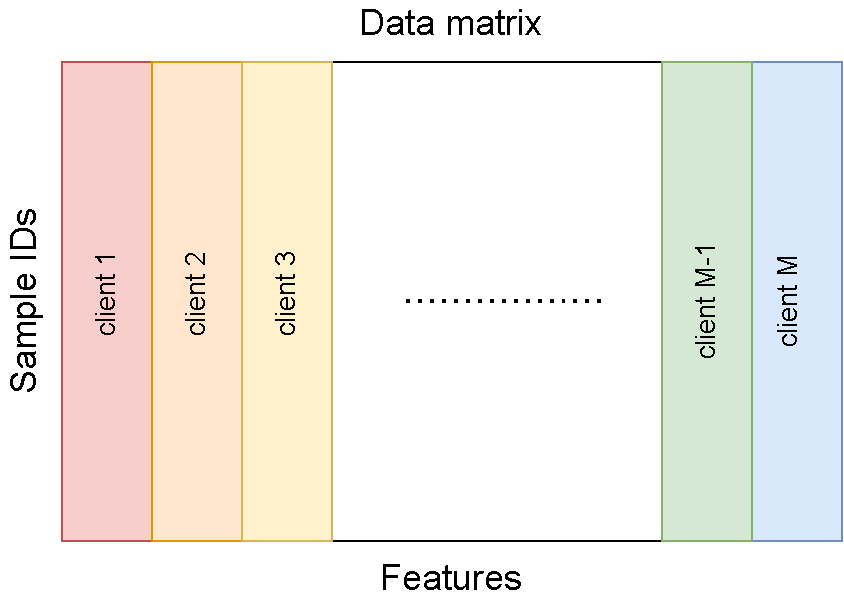
\includegraphics[width=\linewidth]{./figures/vfl_illustration.pdf}
      \captionsetup{justification=centering}
      \caption{Vertical federated learning.}
      \label{fig:vfl}
    \end{subfigure}
    \captionsetup{justification=centering}
    \caption{Characterization of horizontal and vertical federated learning.}
    \label{fig:hfl_and_vfl}
\end{figure}


At the physical level, a federated learning system is often comosed of two components: clients and a central server. The learning process in federated learning can be formulated as a distributed optimization problem, which is also known as federated optimization. As characterized and formalized by~\citet{wang2021field},~\citet{li2020federated} and~\citet{li2019convergence}, there are several important characteristics that distinguish FO from standard machine learning and distributed optimization. 
\begin{assumption}[Governing assumptions for federated optimization] \label{assum:govern}
The following assumptions hold for FO. 
  \begin{itemize}
    \item \textbf{Slow Communication.}  Communication between clients and a central server is assumed to be the main bottleneck and dominates any computational work done at each of the clients. 
    \item \textbf{Data Privacy.} Clients want to keep their local data private, i.e., their data can not be accessed by any other client nor by the central server.
    \item \textbf{Data heterogeneity.} The training data are not independent and identically distributed (i.i.d.). In other words, a client’s local data cannot be regarded as samples drawn from single overall distribution.
    \item \textbf{Partial Participation.} Unlike traditional distributed learning systems, an FL system does not have control over individual client devices, and clients may have limited availability for connection. 
\end{itemize}
\end{assumption}

In this thesis, want to develop an efficient and scalable algorithm for the federated optimization problem, which satisfies these governing assumptions (\autoref{assum:govern}). We study the federated optimization problem from a dual perspective and propose a new algorithm termed federated dual coordinate descent (FedDCD), which is based on a type of coordinate descent method developed by \citet{necoara2017random}. 

The effectiveness of federated learning depends on the active participation of motivated clients. Another important question in federated learning is how to ensure the clients’ long-term engagement, and how to motivate more clients' participation. One possible practical solution is to recompense the participated clients according to their contribution. In this thesis, we want to design fair and efficient contribution valuation techniques for both horizontal and vertical federated learning. Our approach relies on the concepts and tools from structured optimization. We provide a more detailed roadmap in \autoref{sec:1-4}. 



\section{Roadmap} \label{sec:1-5}


